\documentclass[11pt,a4paper]{article}
\usepackage[T1]{fontenc}
\usepackage[utf8]{inputenc}
\usepackage{times}
\usepackage{microtype}
\usepackage{amsmath,amssymb,amsthm}
\usepackage{booktabs}
\usepackage{graphicx}
\usepackage{geometry}
\usepackage{caption}
\usepackage{algorithm}
\usepackage{algpseudocode}
\usepackage{xcolor}
\usepackage[hidelinks]{hyperref}
\geometry{margin=2.6cm}
\captionsetup{font=small,labelfont=bf}

\newtheorem{proposition}{Proposition}
\newtheorem{lemma}{Lemma}
\newtheorem{definition}{Definition}
\newtheorem{remark}{Remark}

\newcommand{\R}{\mathbb{R}}
\newcommand{\E}{\mathbb{E}}
\newcommand{\Prob}{\mathbb{P}}
\newcommand{\dd}{\mathrm{d}}
\newcommand{\sbp}{\mathrm{sbp}}
\newcommand{\dbp}{\mathrm{dbp}}
\newcommand{\glu}{\mathrm{glu}}
\newcommand{\hr}{\mathrm{hr}}

\title{\bfseries The TeleMonitor Risk Model\\[2mm]
\large Formalisation, Learning Algorithm, Attribution and\\
Empirical Evaluation on a Prospective Hospital Cohort}
\author{Nsame Rodrick Ayuni\\[1mm]
\small M2R Data Science \& Artificial Intelligence\\
\small École Nationale Supérieure Polytechnique de Douala}
\date{\today}

\begin{document}
\maketitle

\begin{abstract}
\noindent
This document specifies, derives and evaluates the predictive model at the core of
\textsc{TeleMonitor}, a mobile telemonitoring system for patients living with
hypertension and type~2 diabetes in Douala, Cameroon. We formalise clinical
telemonitoring as \emph{short-horizon forecasting over an irregularly sampled
multivariate physiological stream}, and argue that the formulation itself --- not
the choice of learner --- is where most of the methodological risk lies. We give
a feature map from a sliding window of seven readings into $\R^{16}$, with closed
forms for each descriptor and an explicit, provable guard against the degeneracy
that last-observation-carried-forward imputation induces when a channel is nearly
unobserved. We derive the gradient-boosted tree learner from its second-order
objective, state precisely how absent channels are handled without imputation, and
derive the scalar risk score $R$ as the probability of a disjoint union of
outcomes rather than, as is common, an arbitrary weighted sum.

The model is trained and evaluated on a prospective cohort of 32 inpatients
(366 readings) collected from ward surveillance charts at a public hospital in
Douala. We report three findings that a naive evaluation would have concealed.
First, the conventional \emph{nowcasting} formulation --- label a window by its own
final reading --- is degenerate: the label is a deterministic function of three of
the sixteen features, and the resulting accuracy of $0.863$ measures arithmetic,
not prediction. Second, after reformulating as genuine forecasting, a pooled
alert-detection AUC of $0.754$ collapses to $0.673$ once we restrict to windows in
which glucose was actually measured --- because \emph{whether glucose was ordered}
is itself a 0.698-AUC predictor, encoding which ward the patient occupies rather
than their physiology. Third, a feature ablation that was significant on
distribution-matched synthetic data fails to replicate on real data
($\Delta\mathrm{AUC}=+0.005$, $p=0.058$, 17/30 paired partitions).
We argue that reporting these three negative results is the main scientific
contribution of this chapter, and that the honest operating figure for the
deployed system is an alert sensitivity of $0.58$ at a specificity of $0.79$
against a carry-forward baseline of $0.70/0.66$ --- a system that is useful, and
whose usefulness is bounded in a way we can state.
\end{abstract}

\tableofcontents
\bigskip

\section{Introduction}

\subsection{The clinical setting, and why it is not a standard time-series problem}

Hypertension and type~2 diabetes are managed, not cured. Management is a control
problem: a clinician observes a noisy physiological state at irregular intervals,
adjusts therapy, and waits. The quality of that control is bounded by the
\emph{observation rate}. In high-income settings this rate is lifted by home
devices and electronic records; in Douala it is bounded by whether the patient
returns to the clinic, and by whether anyone wrote the number down.

An earlier retrospective collection for this project made the point quantitatively.
Of 58 patients drawn from consultation records at a Douala public hospital,
49 ($84.5\%$) had exactly one recorded measurement; one patient reached seven, and
those seven spanned 134 days. The median interval between consecutive visits was
1.5 days and the mean was 47.0 days --- a distribution so heavy-tailed that
neither statistic describes a typical patient. No sliding window of any useful
length can be formed from such a record. \emph{The absence of the data is the
problem the system exists to solve}, and it is therefore not a defect of the study
but its premise.

This observation dictated the second collection, from which all results in this
document derive: ward \emph{fiches de surveillance} --- paper charts on which
nursing staff record blood pressure, pulse and, when ordered, capillary glycaemia
twice daily for the duration of an admission. These charts are dense where
consultation records are sparse. They are also, as we show in
Section~\ref{sec:confound}, selected in a way that creates a trap for the
unwary analyst.

\subsection{What is actually being predicted}

A telemonitoring system is not a diagnostic instrument. It does not need to
establish what is wrong with a patient; a clinician does that. It needs to answer
a narrower and more operational question:

\begin{quote}
\itshape Given this patient's recent measurement history, is their next
measurement likely to be one that requires clinical attention?
\end{quote}

This framing has three consequences that run through the whole design. It is
\emph{prospective}: the target lies in the future, not in the window. It is
\emph{decision-theoretic}: the output is consumed by an alerting rule with a
tunable threshold, so calibrated probabilities matter more than hard labels. And
it is \emph{asymmetric}: failing to raise an alert for a patient heading into a
hypertensive crisis is not the same kind of error as raising one for a patient who
turns out to be fine.

\subsection{Contributions}

\begin{enumerate}
\item A precise formalisation of the telemonitoring task as short-horizon
forecasting over an irregularly sampled multivariate stream, with an explicit
feature map and a proof that the minimum-observation guard is necessary rather
than conservative (Section~\ref{sec:features}).

\item A demonstration that the \emph{nowcasting} formulation widely used in
window-based clinical risk modelling is, under threshold-derived labels,
arithmetically degenerate, and a reformulation that removes the degeneracy
(Section~\ref{sec:leakage}).

\item A derivation of the scalar risk score as the probability of a disjoint union
of classes, replacing the ad hoc weighted sums common in the applied literature,
together with the consequence that the score inherits the model's calibration
(Section~\ref{sec:riskscore}).

\item An evaluation protocol that is patient-disjoint, nested, and compared against
the only baseline that matters clinically --- carry-forward persistence
(Section~\ref{sec:protocol}).

\item The identification of \emph{informative missingness as a confound} in
ward-collected physiological data, with a quantification of how much apparent
performance it manufactures (Section~\ref{sec:confound}). To our knowledge this
specific failure mode has not been reported for telemonitoring cohorts assembled
from paper ward charts.

\item A non-replication: a feature-set ablation that was significant on
distribution-matched synthetic cohorts does not reproduce on real data
(Section~\ref{sec:ablation}).

\item A verified deployment path: the trained model is exported to ONNX and shown
to agree with the training-time implementation to $1.8\times10^{-7}$ in
probability, including on inputs containing unobserved channels
(Section~\ref{sec:deploy}).
\end{enumerate}

\subsection{Intellectual inspiration}

Three lines of work shape the design. From \emph{early-warning scores} in acute
care --- NEWS, MEWS and their descendants --- we take the idea that a single scalar,
thresholded, is what a busy clinical workflow can actually act upon, and that the
scalar must be interpretable at the bedside. From \emph{gradient boosting}
\cite{friedman2001,chen2016} we take a learner that handles small tabular
datasets, heterogeneous feature scales, and --- critically for this application ---
missing values as a first-class citizen rather than through imputation. From
\emph{cooperative game theory} \cite{shapley1953,lundberg2017,lundberg2020} we take
an attribution method whose axioms are stated in advance, which matters when the
alternative (gain-based importance) is known to be biased precisely in the regime
we operate in: strongly correlated predictors.

What we add is not a new learner. It is a careful account of what happens when
these tools meet a dataset whose missingness is generated by hospital logistics
rather than by physiology.

\section{Problem formalisation}
\label{sec:formal}

\subsection{The observation process}

Let $\mathcal{P}$ index patients. For patient $p\in\mathcal{P}$ we observe a finite
sequence of \emph{readings}
\[
  \mathcal{O}_p \;=\; \bigl\{(\tau_{p,1}, \mathbf{z}_{p,1}),\,
                             (\tau_{p,2}, \mathbf{z}_{p,2}),\,\dots,\,
                             (\tau_{p,n_p}, \mathbf{z}_{p,n_p})\bigr\},
  \qquad \tau_{p,1} \le \tau_{p,2} \le \cdots \le \tau_{p,n_p},
\]
where $\tau_{p,i}$ is a timestamp and
$\mathbf{z}_{p,i}\in(\R\cup\{\varnothing\})^{4}$ is a vector over the four
measurement channels
\[
  \mathcal{C} \;=\; \bigl(\sbp,\; \dbp,\; \glu,\; \hr\bigr),
\]
systolic and diastolic blood pressure (mmHg), capillary glycaemia
(mmol\,L$^{-1}$) and heart rate (min$^{-1}$). The symbol $\varnothing$ denotes
\emph{not observed}, which is distinct from, and must never be encoded as,
the numeric value zero.

Two properties of $\mathcal{O}_p$ distinguish this from textbook time-series
modelling and drive every subsequent design choice.

\paragraph{(P1) Irregular and channel-dependent sampling.}
The timestamps are not equally spaced, and the observed subset of $\mathcal{C}$
varies from reading to reading. In the cohort studied here, blood pressure and
pulse are recorded at $97.5\%$ and $96.7\%$ of readings respectively, whereas
glycaemia is recorded at only $68.6\%$ --- and, decisively, its presence is
clustered by patient rather than scattered at random.

\paragraph{(P2) Missingness is not ignorable.}
Glycaemia is measured when a clinician orders it. That decision depends on the
admitting diagnosis. The missingness mechanism is therefore neither MCAR nor MAR
given the observed physiology; it is driven by a latent variable (the reason for
admission) that is correlated with the outcome. Section~\ref{sec:confound} shows
that ignoring this inflates apparent performance by roughly eight AUC points.

\subsection{Discretising the index}

Rather than model $\tau$ continuously, we index readings by their rank within the
patient,
\[
  t \;=\; 1,2,\dots,n_p,
\]
and retain the calendar timestamp only for auditing. This is a deliberate
simplification with a stated cost. On a ward chart readings arrive in a
near-regular morning/evening rhythm, so rank and time are close to affinely
related within an admission; across admissions, and in the deployed app where a
patient may log readings erratically, they are not. The model therefore learns
\emph{per-reading} dynamics, not \emph{per-hour} dynamics, and a trend coefficient
must be read as ``change per reading'' rather than ``change per day''.
Section~\ref{sec:limits} returns to this.

\begin{remark}[Morning/evening slots]
Each chart day contributes two readings, a morning ($M$) and an evening ($S$)
slot. Treating them as two elements of the sequence rather than averaging them
doubles the usable sequence length --- the binding constraint in this setting ---
at the cost of folding a genuine circadian component into the within-window
variance. We record the slot explicitly so that a morning-only sensitivity
analysis remains possible; we did not have the statistical power to run it
meaningfully here.
\end{remark}

\section{From readings to features}
\label{sec:features}

\subsection{The sliding window}

Fix a window length $W=7$. For patient $p$ and anchor index $i$ with
$1 \le i \le n_p - W$, define the window
\[
  \mathbf{W}_{p,i} \;=\; \bigl(\mathbf{z}_{p,i},\,\mathbf{z}_{p,i+1},\,\dots,\,
                                \mathbf{z}_{p,i+W-1}\bigr),
\]
and write $x^{(c)}_{1:W}$ for the length-$W$ slice of channel $c\in\mathcal{C}$
inside it. The choice $W=7$ is a compromise: it is long enough for a linear trend
to be estimable against noise, and short enough that a patient with a nine-day
admission still contributes several windows. Since the number of windows a patient
contributes is $n_p - W$, the cost of $W$ is paid in sample size, steeply: raising
$W$ from 7 to 10 would have removed $9$ of our $26$ eligible patients entirely.

\subsection{The descriptor map}

Each channel is summarised by four descriptors, giving
$4\times 4 = 16$ features. Let $\tilde{x}_{1:W}$ denote the channel slice after
the imputation of Section~\ref{sec:locf}, and let
$\bar{x} = W^{-1}\sum_{k=1}^{W}\tilde{x}_k$.

\begin{align}
  \mu(x)        &= \bar{x} &&\text{level} \label{eq:mean}\\[1mm]
  \sigma(x)     &= \Bigl(\tfrac{1}{W}\textstyle\sum_{k=1}^{W}(\tilde{x}_k-\bar{x})^2\Bigr)^{1/2}
                 &&\text{variability} \label{eq:std}\\[1mm]
  \beta(x)      &= \frac{\sum_{k=1}^{W}(k-\bar{k})(\tilde{x}_k-\bar{x})}
                        {\sum_{k=1}^{W}(k-\bar{k})^{2}}
                 &&\text{trend} \label{eq:trend}\\[1mm]
  \lambda(x)    &= \tilde{x}_W &&\text{current level} \label{eq:last}
\end{align}

Three points deserve emphasis.

\paragraph{The standard deviation uses the population convention.}
We divide by $W$, not $W-1$. The window is not a sample drawn from a larger
population whose variance we wish to estimate; it \emph{is} the object being
described. Using $\mathrm{ddof}=0$ also makes $\sigma$ well defined and equal to
zero for a constant window, which the degeneracy analysis below requires.

\paragraph{The trend is an ordinary least-squares slope in closed form.}
Regressing $\tilde{x}$ on $k\in\{1,\dots,W\}$ gives the usual normal-equation
solution, and because the design points are the fixed integers $1,\dots,W$, the
denominator is a constant:
\[
  \sum_{k=1}^{7}(k-4)^2 \;=\; 9+4+1+0+1+4+9 \;=\; 28 .
\]
Hence
\[
  \beta(x) \;=\; \frac{1}{28}\sum_{k=1}^{7}(k-4)\,\tilde{x}_k ,
\]
a fixed linear functional of the window --- one dot product, no iteration, no
matrix inversion. This matters for on-device inference: the entire feature map is
$O(W)$ per channel with no allocation.

\paragraph{The feature vector is ordered canonically.}
\[
  \phi(\mathbf{W}) = \bigl(
  \mu_{\sbp},\sigma_{\sbp},\beta_{\sbp},\lambda_{\sbp},\;
  \mu_{\dbp},\dots,\;
  \mu_{\glu},\dots,\;
  \mu_{\hr},\sigma_{\hr},\beta_{\hr},\lambda_{\hr}\bigr) \in \R^{16}.
\]
This ordering is a contract between the training pipeline, the ONNX graph and the
Dart client. A permutation of it is a silent, catastrophic bug --- the model would
still run and still return plausible probabilities --- so it is asserted in the
export test of Section~\ref{sec:deploy}.

\subsection{Imputation, and why it needs a guard}
\label{sec:locf}

Within a window, gaps in an otherwise observed channel are filled by
last-observation-carried-forward, with a single backward fill to cover a leading
gap:
\[
  \tilde{x}_k \;=\;
  \begin{cases}
    x_k & x_k \ne \varnothing,\\
    \tilde{x}_{k-1} & x_k = \varnothing,\; k>1,\\
    x_{k^\ast} & x_k = \varnothing,\; k=1,\quad k^\ast=\min\{j: x_j\ne\varnothing\}.
  \end{cases}
\]
LOCF is the standard choice for clinical signals because it corresponds to the
assumption a clinician actually makes between measurements: in the absence of new
information, the last value still stands. But applied naively it manufactures
structure out of nothing, and the following makes that precise.

\begin{lemma}[Degeneracy of LOCF under extreme sparsity]
\label{lem:degeneracy}
Suppose channel $c$ has exactly one observed value in the window, at position
$k^\ast$, with value $v$. Then $\tilde{x}_k = v$ for all $k$, and consequently
\[
  \mu = v,\qquad \sigma = 0,\qquad \beta = 0,\qquad \lambda = v .
\]
\end{lemma}

\begin{proof}
For $k \ge k^\ast$ the forward fill propagates $v$; for $k < k^\ast$ the backward
fill assigns $x_{k^\ast}=v$. Hence $\tilde{x}\equiv v$ and $\bar{x}=v$. Then
$\sigma^2 = W^{-1}\sum_k (v-v)^2 = 0$, and
$\beta = \tfrac{1}{28}\sum_k (k-4)(v-v) = 0$. The last value is $\tilde{x}_W=v$.
\end{proof}

The consequence is not that the numbers are wrong but that they are
\emph{indistinguishable from a true clinical finding}. A patient measured once at
$140$ mmHg and a patient measured seven times at exactly $140$ mmHg produce the
identical feature vector $(\mu,\sigma,\beta,\lambda)=(140,0,0,140)$. The second is
a remarkable observation --- perfectly stable pressure over a week. The first is an
absence of information. A model trained on both learns to treat sparsity as
stability, which in a telemonitoring system means learning that \emph{patients who
stop measuring are well}. This is precisely backwards, and precisely the population
such a system exists to catch.

We therefore impose a guard. Let $m_c$ be the number of genuinely observed values
of channel $c$ in the window, and fix $m_{\min}=3$.

\begin{definition}[Guarded descriptor map]
\label{def:guard}
\[
  \bigl(\mu_c,\sigma_c,\beta_c,\lambda_c\bigr) =
  \begin{cases}
    \text{Eqs.~\eqref{eq:mean}--\eqref{eq:last} applied to } \tilde{x}^{(c)},
      & m_c \ge m_{\min},\\[1mm]
    (\textsc{nan},\textsc{nan},\textsc{nan},\textsc{nan}), & m_c < m_{\min}.
  \end{cases}
\]
\end{definition}

The threshold $m_{\min}=3$ is the smallest value at which all four descriptors are
jointly non-degenerate: two observations already determine a line exactly, so
$\beta$ carries no information about fit quality and $\sigma$ is a function of the
single increment; three is the minimum at which variability and trend are
separately identifiable.

Crucially, \textsc{nan} here is a \emph{value the learner understands}, not a
sentinel to be replaced. Section~\ref{sec:nan} explains how gradient-boosted trees
consume it. The alternative --- imputing a cohort mean --- would assert that an
unmeasured patient is an average patient, which is exactly the inference we have
just argued is unsafe.

\subsection{Window admissibility}

A window is retained if and only if the three \emph{vital} channels
$\sbp,\dbp,\hr$ each satisfy $m_c \ge m_{\min}$. Glycaemia is \emph{optional}: a
window in which it was never measured is admitted, with its four descriptors set
to \textsc{nan}.

This asymmetry is a clinical judgement, not a statistical one. Blood pressure and
pulse are taken on every ward round for every patient; their absence indicates a
broken record. Glycaemia is ordered on indication; its absence is ordinary. A rule
requiring all four channels would have discarded $40$ of our $146$ windows and,
because those $40$ belong overwhelmingly to the non-diabetic admissions, would have
removed most of the low-risk end of the label distribution --- turning a balanced
problem into a degenerate one.

\section{The target variable}
\label{sec:target}

\subsection{The labelling functional}

Risk levels are derived from the measured values by a deterministic rule built on
the 2023 European Society of Hypertension grades for blood pressure and the WHO
thresholds for random (non-fasting) plasma glucose. Define
$\ell : (\R\cup\{\varnothing\})^3 \to \{0,1,2,3\}$ by
\begin{equation}
\label{eq:label}
  \ell(s,d,g) =
  \begin{cases}
    3 \ (\textsf{critical}) & s\ge 180 \ \vee\ d\ge 110 \ \vee\ g\ge 14,\\
    2 \ (\textsf{high})     & s\ge 160 \ \vee\ d\ge 100 \ \vee\ g\ge 11,\\
    1 \ (\textsf{moderate}) & s\ge 140 \ \vee\ d\ge 90  \ \vee\ g\ge 8,\\
    0 \ (\textsf{stable})   & \text{otherwise,}
  \end{cases}
\end{equation}
evaluated top-down, with $\varnothing$ never satisfying a comparison. The
disjunction encodes the clinical convention that the worst channel governs: a
patient with normal pressure and a glucose of $15$ mmol\,L$^{-1}$ is critical.

\subsection{A stated blind spot}

Rule~\eqref{eq:label} is monotone upward only. It has no lower thresholds, and
therefore maps hypotension and hypoglycaemia to \textsf{stable}. In the cohort
this is not hypothetical:

\begin{itemize}
\item $32$ readings have $\sbp<90$ or $\dbp<60$; $24$ of them are labelled
      \textsf{stable}. Patient~31 at $71/54$ mmHg with a pulse of $102$ --- a
      textbook shock presentation --- is scored \textsf{stable}.
\item $4$ readings have glucose $<3.9$ mmol\,L$^{-1}$; one, at
      $2.4$ mmol\,L$^{-1}$, is labelled \textsf{stable}.
\end{itemize}

A deployed system that reassures a hypotensive or hypoglycaemic patient is not
merely inaccurate, it is harmful. The defensible fix is a symmetric rule with
lower thresholds; we state the defect here rather than in the limitations because
it affects the \emph{labels}, and hence every number reported in this document.
All results below should be read as describing performance on the upward-risk
problem only.

\subsection{Nowcasting is degenerate}
\label{sec:leakage}

The natural first formulation --- and the one used in the earlier synthetic phase
of this project --- labels a window by the level of its own final reading:
\[
  y^{\text{now}}_{p,i} \;=\; \ell\bigl(s_{p,i+W-1},\, d_{p,i+W-1},\, g_{p,i+W-1}\bigr).
\]

\begin{proposition}[Label leakage under nowcasting]
\label{prop:leak}
Let $\phi(\mathbf{W})$ be the guarded feature map of Definition~\ref{def:guard}.
If all four channels are admissible, then
$y^{\text{now}} = \ell(\lambda_{\sbp}, \lambda_{\dbp}, \lambda_{\glu})$ exactly.
That is, the label is a deterministic function of three of the sixteen features.
\end{proposition}

\begin{proof}
Immediate from $\lambda_c = \tilde{x}^{(c)}_W$ and the definition of
$y^{\text{now}}$, provided the final reading of each channel was observed rather
than carried forward. When it was carried forward, $\lambda_c$ equals the last
observed value and the identity holds up to the carried gap.
\end{proof}

A learner given $\phi$ therefore need only recover three thresholded comparisons.
Empirically, the nowcasting model attains $0.863$ cross-validated accuracy ---
a figure that would look respectable in a results table and that measures nothing
but the model's ability to rediscover Eq.~\eqref{eq:label}. It falls short of
$1.0$ only because of carried-forward finals and tree discretisation.

\begin{remark}
This degeneracy is not an artefact of our particular thresholds. It arises whenever
window-derived labels are computed from values that also enter the feature map, a
pattern common enough in the applied clinical-ML literature that we regard flagging
it as a contribution. The diagnostic is simple: if the label can be written as a
function of the features without reference to any unobserved quantity, the task is
arithmetic rather than inference.
\end{remark}

\subsection{The forecasting formulation}

We therefore define the target one step ahead of the window:
\begin{equation}
\label{eq:target}
  y_{p,i} \;=\; \ell\bigl(s_{p,\,i+W},\, d_{p,\,i+W},\, g_{p,\,i+W}\bigr),
  \qquad 1 \le i \le n_p - W .
\end{equation}
The reading at index $i+W$ contributes to the label and to no feature. The
resulting learning problem is
\[
  \text{estimate } \; \Prob\bigl(y = k \,\big|\, \phi(\mathbf{W})\bigr),
  \qquad k \in \{0,1,2,3\},
\]
which is what an early-warning system requires and what the remainder of this
document evaluates. The cost is sample size: the usable set falls from $175$
windows over $29$ patients to $146$ windows over $26$ patients, since each patient
forfeits one window and patients with exactly $W$ readings forfeit all of theirs.
We regard $146$ honest examples as worth more than $175$ degenerate ones.

\section{The learner}
\label{sec:learner}

\subsection{Why gradient-boosted trees}

With $n=146$ windows and $p=16$ features --- roughly nine samples per feature ---
the model class must be chosen for data efficiency, not expressive capacity. A
recurrent or attention-based sequence model has the wrong inductive bias at this
scale and would require the raw window rather than our 16 summary statistics;
neither is available in quantity. Logistic regression is data-efficient but cannot
represent the interaction between level and trend that clinicians reason with
(``high, and still rising''). Gradient-boosted decision trees occupy the useful
middle: they capture low-order interactions, are invariant to monotone rescaling of
any feature, degrade gracefully under correlated inputs, and --- the property that
decided it here --- treat missing values as a learned routing decision rather than
a preprocessing problem.

\subsection{The additive model and its objective}

Boosting constructs an additive predictor
\begin{equation}
  F^{(K)}(\mathbf{x}) \;=\; \sum_{k=1}^{K} f_k(\mathbf{x}),
  \qquad f_k \in \mathcal{F},
\end{equation}
where $\mathcal{F}$ is the space of regression trees. Each tree is a piecewise
constant function $f(\mathbf{x}) = w_{q(\mathbf{x})}$, with $q$ mapping a feature
vector to one of $T$ leaves and $w\in\R^T$ the leaf weights. The regularised
objective is
\begin{equation}
\label{eq:obj}
  \mathcal{L} \;=\; \sum_{i=1}^{n} \mathrm{loss}\bigl(y_i, F^{(K)}(\mathbf{x}_i)\bigr)
     \;+\; \sum_{k=1}^{K}\Omega(f_k),
  \qquad
  \Omega(f) = \gamma T + \tfrac{1}{2}\lambda\|w\|^2 .
\end{equation}

Trees are added greedily. Writing $\hat{y}^{(k-1)}_i = F^{(k-1)}(\mathbf{x}_i)$
and expanding the loss to second order in the new tree's output,
\[
  \mathcal{L}^{(k)} \simeq \sum_{i=1}^n
     \Bigl[ g_i f_k(\mathbf{x}_i) + \tfrac{1}{2} h_i f_k(\mathbf{x}_i)^2 \Bigr]
     + \Omega(f_k) + \text{const},
\]
with the first- and second-order statistics
\[
  g_i = \partial_{\hat{y}}\,\mathrm{loss}(y_i,\hat{y})\big|_{\hat{y}^{(k-1)}_i},
  \qquad
  h_i = \partial^2_{\hat{y}}\,\mathrm{loss}(y_i,\hat{y})\big|_{\hat{y}^{(k-1)}_i}.
\]
Grouping the sum by leaf, with $I_j = \{i : q(\mathbf{x}_i)=j\}$,
$G_j = \sum_{i\in I_j} g_i$ and $H_j = \sum_{i\in I_j} h_i$, the objective becomes
a sum of independent quadratics in the leaf weights, whose minimiser is
\begin{equation}
\label{eq:leafweight}
  w_j^\star \;=\; -\,\frac{G_j}{H_j + \lambda},
  \qquad\text{giving}\qquad
  \tilde{\mathcal{L}}^{(k)}(q) \;=\; -\tfrac{1}{2}\sum_{j=1}^{T}\frac{G_j^2}{H_j+\lambda}
  \;+\; \gamma T .
\end{equation}
Eq.~\eqref{eq:leafweight} is the \emph{structure score}: a scalar quality measure
for a tree shape $q$ with the weights already optimised out. A candidate split of
leaf $I$ into $I_L \uplus I_R$ is then scored by the reduction it achieves,
\begin{equation}
\label{eq:gain}
  \mathrm{Gain} \;=\; \tfrac{1}{2}\left[
     \frac{G_L^2}{H_L+\lambda} + \frac{G_R^2}{H_R+\lambda}
     - \frac{(G_L+G_R)^2}{H_L+H_R+\lambda}\right] - \gamma ,
\end{equation}
and the split maximising Eq.~\eqref{eq:gain} is taken, provided the gain is
positive. The $-\gamma$ term is intrinsic pruning: a split must pay for the leaf it
creates.

\subsection{The multiclass head}

For $|\mathcal{Y}|=4$ classes the model maintains four additive scores
$F_0,\dots,F_3$ and maps them to probabilities by the softmax
\begin{equation}
\label{eq:softmax}
  \hat{p}_k(\mathbf{x}) \;=\; \frac{\exp F_k(\mathbf{x})}
                                   {\sum_{j=0}^{3}\exp F_j(\mathbf{x})},
\end{equation}
trained under the multinomial cross-entropy
$\mathrm{loss} = -\sum_k \mathbb{1}[y=k]\log \hat p_k$. The derivatives that feed
Eqs.~\eqref{eq:leafweight}--\eqref{eq:gain} take the familiar form
\[
  g_{i,k} = \hat{p}_k(\mathbf{x}_i) - \mathbb{1}[y_i=k],
  \qquad
  h_{i,k} = \hat{p}_k(\mathbf{x}_i)\bigl(1-\hat{p}_k(\mathbf{x}_i)\bigr),
\]
so each boosting round grows one tree per class. By construction
$\hat{p}_k \ge 0$ and $\sum_k \hat{p}_k = 1$: the outputs are a genuine
distribution over the four levels, which is what makes the risk score of
Section~\ref{sec:riskscore} a probability rather than an index.

\subsection{Learning the route for an unobserved channel}
\label{sec:nan}

This is the property that makes the guard of Definition~\ref{def:guard} practical.
At each internal node, the tree stores a split $(\text{feature } m,\ \text{threshold } \theta)$
\emph{and} a default direction $\delta\in\{L,R\}$. Routing is
\[
  \text{child}(\mathbf{x}) =
  \begin{cases}
    L & x_m \ne \textsc{nan} \ \wedge\ x_m < \theta,\\
    R & x_m \ne \textsc{nan} \ \wedge\ x_m \ge \theta,\\
    \delta & x_m = \textsc{nan}.
  \end{cases}
\]
The default $\delta$ is not a convention; it is \emph{fitted}. During split
enumeration the algorithm evaluates Eq.~\eqref{eq:gain} twice --- once sending all
missing-valued instances left, once right --- and keeps whichever scores higher.
The tree thus learns, from the training data, what an absent glycaemia channel
should imply.

Two consequences follow. The useful one: a hypertensive patient who never logs a
glucose reading still receives a prediction, with no value invented on their
behalf. The dangerous one: whatever the \emph{absence} of glycaemia correlates with
in the training data will be learned as signal. Section~\ref{sec:confound} shows
that in this cohort that correlation is an artefact of ward allocation, and
quantifies the damage.

\subsection{Class weighting}

The four levels are unequally frequent and unequally costly. Each training instance
receives a weight
\begin{equation}
\label{eq:weights}
  w(y) \;=\; \underbrace{\frac{n}{4\,n_y}}_{\text{inverse frequency}} \times\;
  \kappa_y, \qquad
  \kappa = (1,\,1,\,1.5,\,3) ,
\end{equation}
where $n_y$ is the count of class $y$. The first factor removes the frequency
imbalance; the second encodes the asymmetry of clinical cost, penalising a missed
\textsf{critical} three times more than a missed \textsf{stable}. The weights enter
the objective through $g_i$ and $h_i$ and therefore propagate into both the leaf
weights and the split gains. We stress that $\kappa$ is a \emph{value judgement},
not an estimate; it is stated here so that a clinician can disagree with it
explicitly and a reviewer can vary it.

\section{The risk score}
\label{sec:riskscore}

\subsection{Derivation}

The application needs one number per patient: a dial a clinician can threshold and
a patient can watch. A common practice in applied work is to form a weighted sum
of class probabilities with hand-chosen coefficients, e.g.
$R = 0.1\hat p_1 + 0.5 \hat p_2 + 1.0\hat p_3$. Such a score is uninterpretable ---
it is not a probability of anything --- and its coefficients are unfalsifiable.

We instead define the \emph{actionable} event. Let
\[
  A \;=\; \{\,y = \textsf{high}\,\} \cup \{\,y=\textsf{critical}\,\}
\]
be the event that the next reading warrants clinical attention. The two
constituent events are mutually exclusive, being distinct values of a single
categorical variable, so finite additivity of probability gives immediately
\begin{equation}
\label{eq:risk}
  R(\mathbf{x}) \;\equiv\; \Prob\bigl(A \mid \mathbf{x}\bigr)
   \;=\; \Prob(y=2\mid\mathbf{x}) + \Prob(y=3\mid\mathbf{x})
   \;\approx\; \hat p_2(\mathbf{x}) + \hat p_3(\mathbf{x}).
\end{equation}

The apparent ``weighted sum with weights $(0,0,1,1)$'' is therefore not a choice at
all. It is the only expression consistent with the probability axioms once the
event $A$ has been named, and naming $A$ is a clinical decision made in the open.

\begin{proposition}[Properties of $R$]
$R$ takes values in $[0,1]$; it is invariant to any relabelling that preserves the
partition $\{0,1\}\,|\,\{2,3\}$; and if $\hat p$ is calibrated for the four-class
problem then $R$ is calibrated for the binary event $A$.
\end{proposition}

\begin{proof}
The range and invariance are immediate from $\sum_k \hat p_k = 1$ and
Eq.~\eqref{eq:risk}. For calibration, suppose
$\Prob(y=k \mid \hat p = q) = q_k$ for each $k$. Then
$\Prob(A \mid \hat p = q) = q_2 + q_3 = R$, which is the definition of calibration
for the induced binary problem.
\end{proof}

The last clause is why the derivation matters practically: it licenses the
threshold table of Section~\ref{sec:results}, in which a cut at $R\ge 0.6$ may be
read as ``alert when the estimated chance of an actionable next reading exceeds
$60\%$''. No weighted-sum index supports that sentence.

\subsection{Thresholding and the operating point}

Alerting is the decision rule $\mathbb{1}[R \ge \theta]$. Choosing $\theta$ is a
cost trade-off, not a modelling question: in a service where a false alert costs a
phone call and a missed alert costs a stroke, $\theta$ belongs low. We report the
whole curve and let the operator choose, which is also the only honest way to
present a model whose discrimination is moderate.

\section{Evaluation protocol}
\label{sec:protocol}

\subsection{Why random splitting is invalid here}

Consecutive windows of one patient share $W-1 = 6$ of their seven readings. Two
such windows are near-duplicates. Under a random train/test split, a patient's
windows land on both sides, and the test set measures memorisation of individuals
rather than generalisation to new ones. We therefore use \textbf{GroupKFold} with
the patient as the group: every window of a patient is confined to a single fold,
so each evaluation asks the operationally correct question --- \emph{how will this
model behave on a patient it has never seen?}

With $26$ eligible patients we use $5$ folds, giving $5$--$6$ held-out patients per
fold.

\subsection{Nested cross-validation}

Selecting hyperparameters by the same cross-validation that reports the score is
optimistically biased, and at $n=146$ the bias is not small. We therefore nest:
within each outer training fold, a 4-fold patient-disjoint inner loop selects
$(\text{n\_estimators}, \text{max\_depth}, \text{learning\_rate},
\text{min\_child\_weight}, \lambda)$ by macro-$F_1$; the chosen configuration is
refitted on the whole outer training fold and applied once to the untouched outer
test fold. Every number in Table~\ref{tab:multiclass} is produced this way.
The configurations selected across the five outer folds were stable --- depth $2$
in four of five, learning rate $0.05$ in all five --- which is itself evidence that
the small sample is driving the model towards simplicity.

\subsection{Baselines}

Two baselines are reported, and the second is the one that matters.

\paragraph{Majority class.} Predict $\arg\max_k n_k$ always. This bounds below
anything worth reporting.

\paragraph{Persistence (carry-forward).} Predict that the next reading has the same
level as the last observed one:
$\hat y^{\text{pers}} = \ell(\lambda_{\sbp},\lambda_{\dbp},\lambda_{\glu})$.
This is what a clinician does by default and what a system with no model at all
would do. \emph{A learned model that does not beat persistence has no reason to
exist}, and we hold the model to that standard throughout.

\subsection{Paired comparison across fold partitions}

Comparing two feature sets by a single cross-validated score confounds the
comparison with the particular partition of patients into folds. We instead draw
$30$ independent random partitions of the patients, evaluate both variants under
each, and test the paired differences with a Wilcoxon signed-rank test. This
controls the partition as a blocking factor and is the procedure used for the
ablation in Section~\ref{sec:ablation}.

\section{Results}
\label{sec:results}

\subsection{The cohort}

\begin{table}[htbp]
\centering
\caption{Prospective cohort, Douala public hospital ward charts.}
\label{tab:cohort}
\small
\begin{tabular}{lr}
\toprule
Patients & 32 \\
Readings & 366 \\
Age (years) & 17--86 (mean $50.7$, SD $16.8$) \\
Sex & 18 F / 14 M \\
Readings per patient & median 12 (range 5--18) \\
Observation slots & morning and evening \\
\midrule
\multicolumn{2}{l}{\emph{Channel availability}}\\
\quad Systolic / diastolic pressure & $357/366$ \quad($97.5\%$) \\
\quad Heart rate & $354/366$ \quad($96.7\%$) \\
\quad Capillary glycaemia & $251/366$ \quad($68.6\%$) \\
\midrule
\multicolumn{2}{l}{\emph{Windows ($W=7$, forecasting target)}}\\
\quad Admissible windows & 146 \\
\quad Contributing patients & 26 \\
\quad With glycaemia observed & 106 \\
\quad With glycaemia absent (\textsc{nan} branch) & 40 \\
\midrule
\multicolumn{2}{l}{\emph{Target distribution over the 146 windows}}\\
\quad \textsf{stable} / \textsf{moderate} / \textsf{high} / \textsf{critical}
  & $41$ / $38$ / $25$ / $42$ \\
\bottomrule
\end{tabular}
\end{table}

\subsection{Four-class forecasting}

\begin{table}[htbp]
\centering
\caption{Four-class next-reading forecasting. Nested, patient-disjoint
cross-validation; no hyperparameter selection on the reported folds.}
\label{tab:multiclass}
\small
\begin{tabular}{lccc}
\toprule
 & Accuracy & Balanced accuracy & Macro-$F_1$ \\
\midrule
Majority class            & $0.288$ & $0.250$ & $0.112$ \\
Persistence (carry-forward)& $0.452$ & $0.439$ & $0.439$ \\
\textbf{XGBoost (nested CV)} & $\mathbf{0.514}$ & $\mathbf{0.479}$ & $\mathbf{0.456}$ \\
\bottomrule
\end{tabular}
\end{table}

The model exceeds persistence on all three summaries, by $6.2$, $4.0$ and $1.7$
points respectively. The margin is real but modest, and we decline to dress it up:
predicting \emph{which of four grades} a patient's next reading will fall into is
substantially harder than predicting whether it will cross an action threshold, and
the four-class figures are reported mainly for completeness.

\subsection{The operational task: alert or not}

Collapsing to the actionable event $A$ of Eq.~\eqref{eq:risk} gives the problem the
deployed system actually solves.

\begin{table}[htbp]
\centering
\caption{Binary alert detection, $y = \mathbb{1}[\text{next reading is high or
critical}]$. \emph{Pooled} uses all 146 windows; \emph{primary} restricts to the
106 windows in which glycaemia was measured (see Section~\ref{sec:confound}).}
\label{tab:binary}
\small
\begin{tabular}{llcc}
\toprule
Analysis & Model & ROC-AUC & PR-AUC \\
\midrule
Pooled ($n=146$, prevalence $0.459$)
  & XGBoost                      & $0.754$ & $0.693$ \\
  & Persistence                  & $0.680$ & $0.583$ \\
  & \emph{``was glycaemia ordered?'' alone} & \emph{$0.698$} & --- \\
\midrule
\textbf{Primary} ($n=106$, prevalence $0.594$)
  & \textbf{XGBoost}             & $\mathbf{0.673}$ & $\mathbf{0.771}$ \\
  & Persistence                  & $0.606$ & $0.652$ \\
  & Blood pressure + pulse only  & $0.626$ & $0.729$ \\
\bottomrule
\end{tabular}
\end{table}

\begin{table}[htbp]
\centering
\caption{Operating points of the risk score $R$ on the pooled set. The operator
chooses $\theta$; the table is the menu.}
\label{tab:operating}
\small
\begin{tabular}{lcccc}
\toprule
Threshold $\theta$ & Sensitivity & Specificity & PPV & Alerts per 100 windows \\
\midrule
$0.30$ & $0.761$ & $0.532$ & $0.580$ & $60.3$ \\
$0.40$ & $0.642$ & $0.696$ & $0.642$ & $45.9$ \\
$0.50$ & $0.582$ & $0.785$ & $0.696$ & $38.4$ \\
$0.60$ & $0.507$ & $0.835$ & $0.723$ & $32.2$ \\
$0.70$ & $0.403$ & $0.911$ & $0.794$ & $23.3$ \\
\midrule
Persistence & $0.701$ & $0.658$ & $0.635$ & $50.7$ \\
\bottomrule
\end{tabular}
\end{table}

Table~\ref{tab:operating} is the most useful object in this document. It shows
that at $\theta=0.3$ the model matches persistence's sensitivity while remaining
below it in alert volume, and that moving up the curve buys precision at a steep
cost in recall. For a service in Douala, where a false alert consumes a phone call
and a missed deterioration may consume a hospital bed, we would deploy at
$\theta\approx 0.35$--$0.40$ and revisit once prospective alert outcomes are
available.

\section{Informative missingness as a confound}
\label{sec:confound}

This section reports the principal methodological finding of the study.

\subsection{The observation}

The pooled alert model attains ROC-AUC $0.754$. Before attributing that to
physiology, consider the single binary variable
\[
  o \;=\; \mathbb{1}\bigl[\text{glycaemia was measured at all in this window}\bigr].
\]
In the cohort,
\[
  \Prob(A \mid o=1) = 0.594 \ (n=106),
  \qquad
  \Prob(A \mid o=0) = 0.100 \ (n=40),
\]
so that $o$ \emph{on its own}, with no physiological information whatsoever,
achieves ROC-AUC $0.698$ --- within $0.056$ of the full sixteen-feature model.

\subsection{The mechanism}

The explanation is logistical, not biological. Capillary glycaemia is ordered when
the admitting team suspects or is managing diabetes. Diabetic and hypertensive
admissions therefore carry an observed glucose channel \emph{and} a high rate of
threshold-crossing readings. Admissions for infection and other acute non-metabolic
causes carry no glucose order \emph{and} largely normal pressures. The missingness
indicator is thus a proxy for the admitting ward.

Because the learner fits a default routing direction for \textsc{nan}
(Section~\ref{sec:nan}), it can and does exploit this. The mechanism that makes the
model robust to absent channels in deployment is the same mechanism that lets it
cheat in evaluation. Both facts follow from the same line of code.

\subsection{Why this matters for deployment}

In the hospital, $o=0$ predicts low risk because it means ``admitted for something
else''. In the deployed app, $o=0$ will mean ``this patient did not log a glucose
reading'', which carries no such implication --- indeed, under the degeneracy
argument of Lemma~\ref{lem:degeneracy}, patients who stop measuring are
disproportionately those drifting out of engagement with care. A model that has
learned $o=0 \Rightarrow$ low risk would be \emph{anti-correlated} with truth in
exactly the subpopulation the system is built for. This is a distribution shift
between the training environment and the deployment environment that no amount of
additional ward data would fix.

\subsection{The remedy, and its cost}

We therefore designate as \emph{primary} the analysis restricted to windows with an
observed glucose channel ($n=106$, $18$ patients). Within that stratum the model
attains ROC-AUC $0.673$ against a persistence baseline of $0.606$
(Table~\ref{tab:binary}). The $0.081$-point drop from the pooled figure is the
portion of apparent performance that was manufactured by the missingness pattern.

Within-stratum performance for the $40$ glucose-absent windows cannot be assessed:
with a prevalence of $0.10$ there are only four positive cases, and the resulting
estimate (ROC-AUC $0.514$) carries no information. Establishing whether the model
is useful for patients who never measure glycaemia requires a cohort enriched for
hypertensive non-diabetics, and is stated as future work.

\begin{remark}[Generalisation of the finding]
Any cohort assembled from clinical records inherits the ordering decisions of the
clinicians who generated it. Where a channel's presence is correlated with the
outcome through a latent allocation variable, a learner with native missing-value
handling will discover that correlation, and a pooled evaluation will reward it.
The diagnostic is cheap and we recommend it as routine: \emph{evaluate the
missingness mask alone as a predictor}. If its AUC approaches the model's, the
model's headline number is not measuring what it appears to.
\end{remark}

\section{Feature attribution}
\label{sec:shap}

\subsection{Why not gain}

The split-gain importance of Eq.~\eqref{eq:gain}, summed over nodes, is the default
diagnostic shipped with boosting libraries. It is unsuitable here. Gain is awarded
to whichever of several correlated features happens to be selected at a node; the
others, though equally informative, receive nothing. In this cohort
\[
  \mathrm{corr}(\mu_{\sbp},\,\mu_{\dbp}) = 0.895,
  \qquad
  \mathrm{corr}(\mu_{\sbp},\,\lambda_{\sbp}) = 0.835,
\]
so the arbitrariness is severe. Gain is also not additive with respect to a
prediction: it describes the fitted ensemble, not any particular patient's score,
and so cannot answer the question a clinician asks --- \emph{why did this patient
get this number?}

\subsection{Shapley values}

We use the Shapley value from cooperative game theory. For a prediction
$f(\mathbf{x})$ and feature set $M = \{1,\dots,16\}$, the contribution of feature
$m$ is the average marginal contribution over all orderings in which it could be
added:
\begin{equation}
\label{eq:shapley}
  \varphi_m(f,\mathbf{x}) \;=\;
  \sum_{S \subseteq M\setminus\{m\}}
  \frac{|S|!\,\bigl(|M|-|S|-1\bigr)!}{|M|!}
  \Bigl[ f_{S\cup\{m\}}(\mathbf{x}) - f_{S}(\mathbf{x}) \Bigr],
\end{equation}
where $f_S$ is the model's expected output given only the features in $S$. The
Shapley value is the unique attribution satisfying local accuracy
($f(\mathbf{x}) = \varphi_0 + \sum_m \varphi_m$), missingness (a feature with no
effect receives zero) and consistency (if a feature's marginal contribution does
not decrease under a model change, its attribution does not decrease).
Consistency is the axiom gain violates.

The sum in Eq.~\eqref{eq:shapley} has $2^{|M|}$ terms, which for $|M|=16$ is
$65\,536$ per prediction per class --- feasible but wasteful. \textsc{TreeSHAP}
\cite{lundberg2020} computes the exact values for tree ensembles in
$O(T L D^2)$ time ($T$ trees, $L$ leaves, $D$ depth) by propagating subset
weightings down each path, which for our ensemble is milliseconds.

\subsection{What the model uses}

\begin{table}[htbp]
\centering
\caption{Global attribution, mean $|\varphi_m|$ over the 146 windows and four
classes, with the gain-based ranking for comparison. A positive rank shift means
gain \emph{under}-ranks the feature.}
\label{tab:shap}
\small
\begin{tabular}{lrrrr}
\toprule
Feature & mean $|\varphi|$ & SHAP rank & Gain rank & Shift \\
\midrule
$\sigma_{\glu}$ \; (glucose variability) & $0.280$ & 1 & 1 & $0$ \\
$\mu_{\sbp}$ \; (systolic level)         & $0.189$ & 2 & 3 & $+1$ \\
$\beta_{\hr}$ \; (pulse trend)           & $0.184$ & 3 & 2 & $-1$ \\
$\mu_{\glu}$ \; (glucose level)          & $0.160$ & 4 & 4 & $0$ \\
$\beta_{\glu}$ \; (glucose trend)        & $0.134$ & 5 & 13 & $\mathbf{+8}$ \\
$\sigma_{\dbp}$                          & $0.132$ & 6 & 5 & $-1$ \\
$\beta_{\sbp}$                           & $0.110$ & 7 & 11 & $+4$ \\
$\sigma_{\hr}$                           & $0.109$ & 8 & 6 & $-2$ \\
$\lambda_{\sbp}$                         & $0.101$ & 9 & 10 & $+1$ \\
$\lambda_{\glu}$                         & $0.095$ & 10 & 9 & $-1$ \\
\quad\vdots & & & & \\
$\mu_{\dbp}$ \; (diastolic level)        & $0.077$ & 15 & 7 & $\mathbf{-8}$ \\
$\lambda_{\hr}$                          & $0.035$ & 16 & 14 & $-2$ \\
\bottomrule
\end{tabular}
\end{table}

Three readings of Table~\ref{tab:shap} are worth recording.

\paragraph{Glucose variability dominates.} $\sigma_{\glu}$ is the single most
influential feature, ahead of every blood-pressure descriptor. Clinically this is
coherent: glycaemic \emph{instability} --- swinging between $5$ and $22$
mmol\,L$^{-1}$ within a week, as several patients in this cohort do --- is a
recognised marker of poor control and impending decompensation, and it is
information a single spot measurement cannot carry. It is also the clearest
justification in the whole study for computing descriptors over a window rather
than feeding the latest reading alone.

\paragraph{Gain and SHAP disagree exactly where the theory predicts.}
$\mu_{\dbp}$ is ranked 7th by gain and 15th by SHAP, an eight-place demotion. Given
$\mathrm{corr}(\mu_{\sbp},\mu_{\dbp}) = 0.895$, this is the correlation artefact in
its textbook form: diastolic level is chosen at splits because it is nearly
interchangeable with systolic level, and is credited for work that systolic level
would have done equally well. The reverse happens to $\beta_{\glu}$, which gain
under-ranks by eight places. Had we reported gain, we would have told the reader
that diastolic pressure matters twice as much as glucose trend; the opposite is
true.

\paragraph{Different classes are driven by different channels.} Per-class
attribution gives, for the top three contributors of each:
\begin{center}
\small
\begin{tabular}{ll}
\toprule
\textsf{stable}   & $\mu_{\glu}$, $\mu_{\sbp}$, $\sigma_{\glu}$ \\
\textsf{moderate} & $\beta_{\hr}$, $\sigma_{\sbp}$, $\sigma_{\dbp}$ \\
\textsf{high}     & $\mu_{\sbp}$, $\beta_{\sbp}$, $\sigma_{\dbp}$ \\
\textsf{critical} & $\sigma_{\glu}$, $\beta_{\hr}$, $\mu_{\hr}$ \\
\bottomrule
\end{tabular}
\end{center}
The pattern is interpretable. \textsf{high} is a blood-pressure phenomenon, driven
by systolic level and its trend. \textsf{critical} is a glycaemic and
haemodynamic one, driven by glucose instability and rising pulse. \textsf{moderate}
is driven almost entirely by variability terms --- it is the class the model
recognises by the \emph{absence} of a settled state, which is both plausible and a
warning that it is the hardest class to call, as its $F_1$ of $0.156$ in the
unnested run confirms.

\begin{figure}[htbp]
\centering
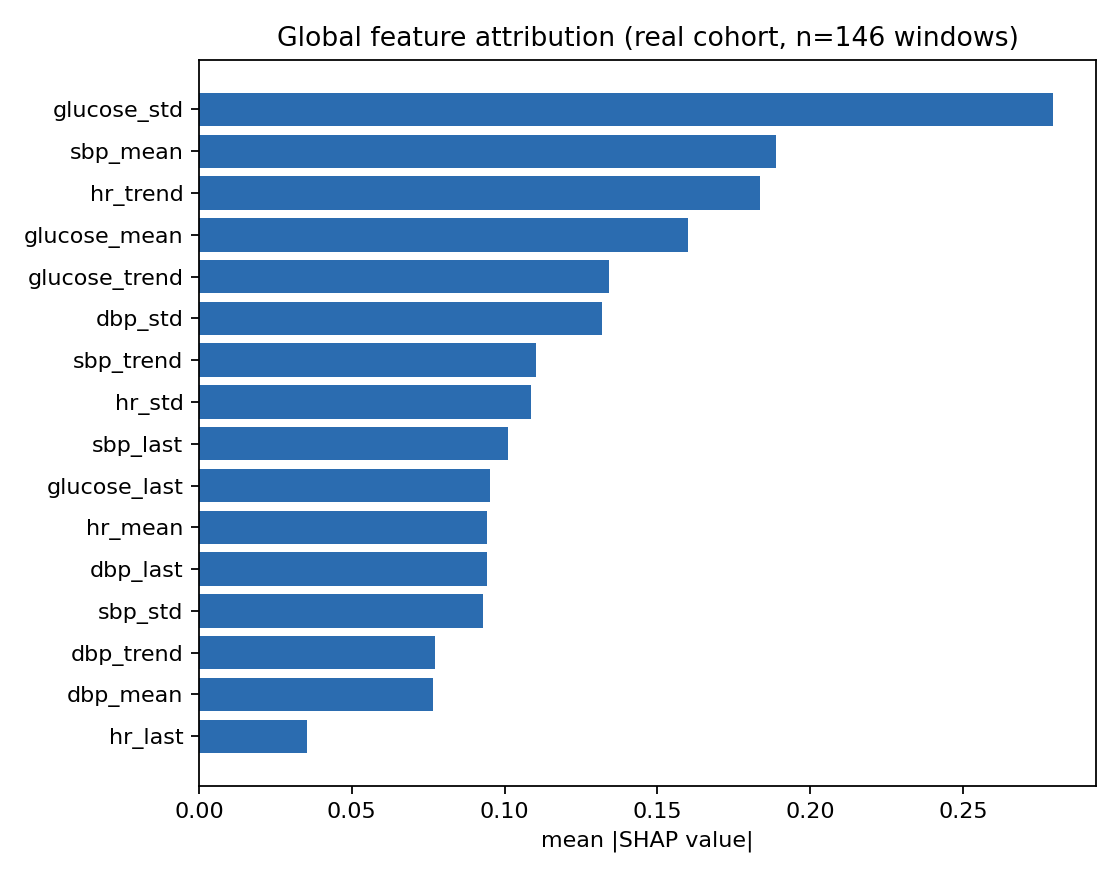
\includegraphics[width=0.78\textwidth]{fig_shap_global.png}
\caption{Global feature attribution on the real cohort. Mean absolute Shapley value
over 146 windows and four output classes.}
\end{figure}

\begin{figure}[htbp]
\centering
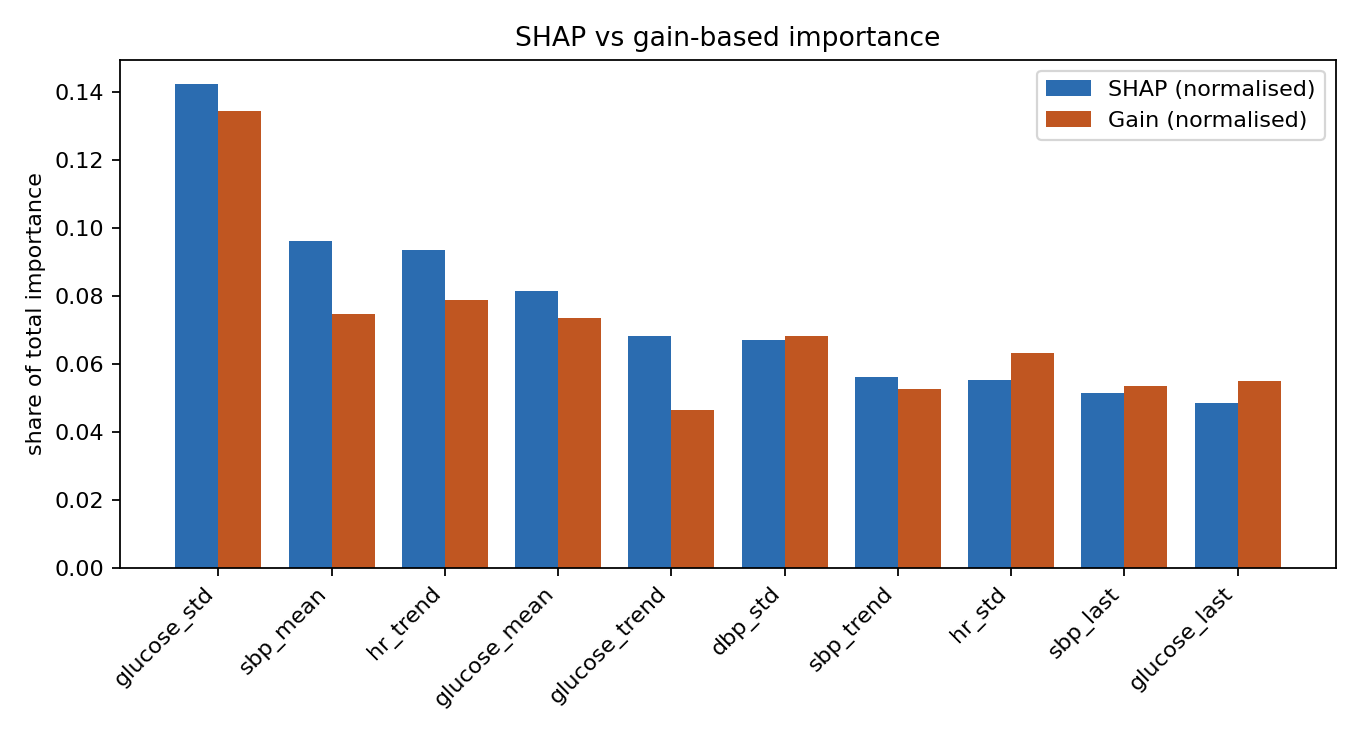
\includegraphics[width=0.92\textwidth]{fig_shap_vs_gain.png}
\caption{Shapley attribution against split-gain importance for the ten most
influential features, each normalised to a share of total importance. The
disagreements are concentrated in the strongly correlated blood-pressure
descriptors.}
\end{figure}

\begin{figure}[htbp]
\centering
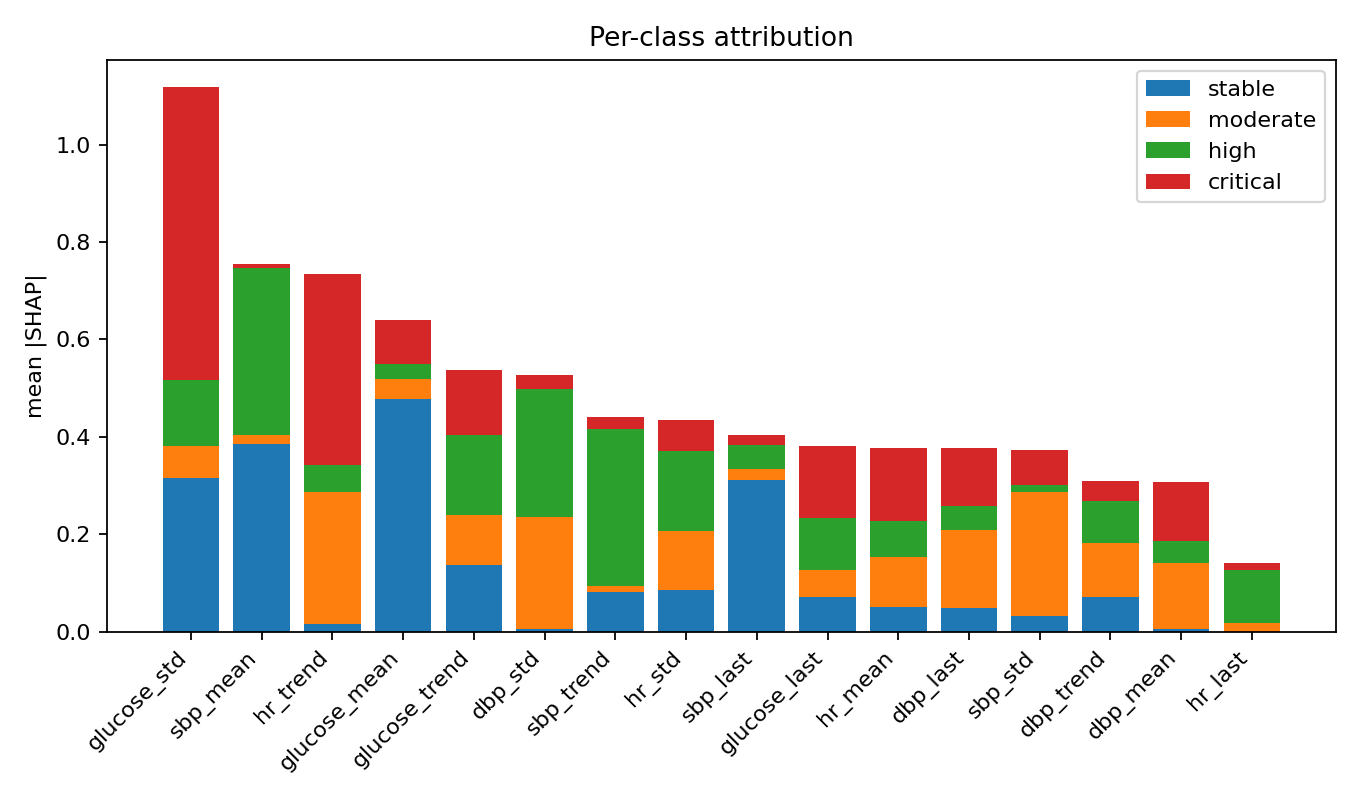
\includegraphics[width=0.92\textwidth]{fig_shap_per_class.png}
\caption{Per-class decomposition of the attribution. Features are ordered by
overall influence; the stacked segments show how that influence divides between the
four predicted levels.}
\end{figure}

\section{Ablation: a non-replication}
\label{sec:ablation}

An earlier phase of this project, conducted on synthetic cohorts calibrated to the
real marginal distributions, found that the full sixteen-feature set significantly
outperformed a reduced set. Across 20 cohorts of 120 simulated patients, accuracy
was $0.892$ versus $0.879$ and precision $0.878$ versus $0.858$, both at
$p = 0.0001$ under a paired Wilcoxon test, with the benefit falling on precision
rather than recall.

That result does not replicate on real data. Table~\ref{tab:ablation} compares the
full descriptor set against a reduced set containing only level and current value
($\mu_c, \lambda_c$ for each channel), over $30$ independent random partitions of
the $18$ patients in the primary stratum.

\begin{table}[htbp]
\centering
\caption{Feature-set ablation on the primary stratum, $30$ paired patient-level
fold partitions.}
\label{tab:ablation}
\small
\begin{tabular}{lcc}
\toprule
Feature set & ROC-AUC (mean $\pm$ SD) & Wins / 30 \\
\midrule
Full 16 ($\mu,\sigma,\beta,\lambda$) & $0.675 \pm 0.019$ & 13 \\
Reduced 8 ($\mu,\lambda$)            & $0.680 \pm 0.013$ & 17 \\
\midrule
\multicolumn{3}{l}{Paired difference $+0.005$; Wilcoxon signed-rank $p = 0.058$} \\
\bottomrule
\end{tabular}
\end{table}

The difference is not significant, and its sign is opposite to the synthetic
finding. We draw the conservative conclusion: at $n=106$ windows over $18$
patients, this study is \emph{underpowered to resolve a difference of five
thousandths of an AUC point}, and no claim should be made in either direction.
We retain the sixteen-feature set, for three reasons: it is the interface already
deployed in the mobile client; the SHAP analysis shows the dispersion and trend
descriptors carrying genuine, interpretable influence
(Table~\ref{tab:shap}) even if that influence does not resolve into a measurable
AUC gain; and discarding features on a non-significant result would itself be a
selection decision made on test data.

We record this non-replication prominently because it is the kind of result that
usually disappears. Synthetic data calibrated to real marginals reproduces the
first moments of a cohort but not its dependence structure, its measurement
protocol, or its missingness mechanism --- and feature-level conclusions evidently
depend on all three. The practical lesson is that \emph{a synthetic ablation is a
hypothesis, not a finding}.

\section{Deployment}
\label{sec:deploy}

\subsection{On-device inference, and why}

Inference runs on the patient's handset, not on a server. The reasons are
specific to the setting rather than architectural fashion. Mobile data in Douala is
metered and intermittent, and a risk score that requires connectivity is
unavailable exactly when a patient is at home and unwell. Round-trip latency to a
server would make the score feel detached from the act of entering a reading.
And physiological measurements never leaving the device is a materially stronger
privacy position than any transport encryption.

The cost is that the model must fit the constraints of a phone and must be
expressible in a format the Dart runtime can load. The trained ensemble is
$119.4$~KB.

\subsection{ONNX export and the parity test}

The model is exported to ONNX, an interchange format that represents the tree
ensemble as a graph of typed operators (\texttt{TreeEnsembleClassifier} followed by
a softmax), decoupled from the Python library that produced it. ONNX is a
\emph{serialisation}, not a compression or an approximation: exporting does not
quantise weights or prune trees, and any numerical difference comes only from
floating-point evaluation order.

That claim is not assumed, it is tested. We evaluate the exported graph under
\texttt{onnxruntime} on all $146$ real feature vectors --- including the $40$ that
contain a \textsc{nan} glycaemia channel, which exercise the learned default
routing of Section~\ref{sec:nan} --- and compare against the training-time
implementation.

\begin{table}[htbp]
\centering
\caption{ONNX parity on the full real feature matrix.}
\label{tab:parity}
\small
\begin{tabular}{lr}
\toprule
Rows evaluated & $146$ \\
\quad of which contain an unobserved channel & $40$ \\
Max $|\Delta \hat p|$ over all rows and classes & $1.788\times 10^{-7}$ \\
Mean $|\Delta \hat p|$ & $2.394\times 10^{-8}$ \\
Max $|\Delta \hat p|$ restricted to \textsc{nan} rows & $1.192\times 10^{-7}$ \\
Max $|\Delta R|$ for the deployed risk score & $1.788\times 10^{-7}$ \\
Agreement of $\arg\max_k \hat p_k$ & $100.00\%$ \\
\bottomrule
\end{tabular}
\end{table}

The residual is at the level of single-precision rounding, which is what it should
be: the export is faithful, and --- the point of including the \textsc{nan} rows ---
the learned missing-value routes survive serialisation. A displayed risk score of
$62\%$ on the handset is the same number the evaluation of
Section~\ref{sec:results} scored.

\subsection{The inference path in the client}

\begin{algorithm}[htbp]
\caption{On-device risk assessment}
\label{alg:infer}
\begin{algorithmic}[1]
\Require patient's stored readings, newest last
\State $\mathcal{W} \gets$ last $W=7$ readings
\If{$|\mathcal{W}| < W$} \State \Return \textsc{Insufficient history} \EndIf
\For{$c \in (\sbp,\dbp,\glu,\hr)$}
  \State $m_c \gets$ number of observed values of $c$ in $\mathcal{W}$
  \If{$c$ is vital \textbf{and} $m_c < 3$} \State \Return \textsc{Insufficient data} \EndIf
  \If{$m_c \ge 3$}
     \State $\tilde x \gets \textsc{Locf}(x^{(c)})$;
            emit $\bigl(\mu,\sigma,\beta,\lambda\bigr)$ by Eqs.~\eqref{eq:mean}--\eqref{eq:last}
  \Else
     \State emit $(\textsc{nan},\textsc{nan},\textsc{nan},\textsc{nan})$
  \EndIf
\EndFor
\State $\mathbf{x} \gets$ the 16 features in canonical order
\State $\hat p \gets \textsc{OnnxRun}(\mathbf{x})$
\State $R \gets \hat p_2 + \hat p_3$ \Comment{Eq.~\eqref{eq:risk}}
\State $\text{completeness} \gets \bigl(\sum_c m_c\bigr) / (4W)$
\State \Return $(\arg\max_k \hat p_k,\; R,\; \text{completeness})$
\end{algorithmic}
\end{algorithm}

The completeness figure is surfaced in the interface alongside the score. A patient
whose assessment rests on twelve of a possible twenty-eight observations should be
told so, and a clinician reviewing the roster should be able to see at a glance
which scores are thin. This is a deliberate refusal to present a single unqualified
number.

\section{What is new here}
\label{sec:novelty}

It is worth being exact about the claim, because overstating it is the easiest way
to lose a viva.

\paragraph{Not new.} Gradient boosting; sliding-window descriptors; Shapley
attribution; ONNX deployment; threshold-based cardiometabolic risk grading. Every
component is standard, and deliberately so: a thesis that introduced a novel
learner \emph{and} a novel clinical application would be unable to attribute its
results to either.

\paragraph{New, in combination and in setting.}
\begin{enumerate}
\item \textbf{An empirical characterisation of why longitudinal cardiometabolic
modelling fails on Cameroonian consultation records, paired with a demonstration
that it succeeds on ward charts from the same hospital.} Cohort~A: 58 patients,
$84.5\%$ with a single reading, effectively zero admissible windows. Cohort~B: 32
patients, 175 admissible windows. Same institution, same conditions, same month.
The contrast localises the obstacle in the follow-up process rather than in the
disease or the patients, which is precisely the obstacle a telemonitoring
application is positioned to remove.

\item \textbf{The identification and quantification of glucose-ordering
missingness as a confound in ward-derived cardiometabolic cohorts.} We are not
aware of this being reported for this data source, and the diagnostic we propose
--- scoring the missingness mask alone --- is cheap enough to become routine.

\item \textbf{A deployed system that degrades gracefully to the channels a patient
actually measures}, by learned \textsc{nan} routing under an explicit
anti-degeneracy guard with a stated proof, rather than by imputation.

\item \textbf{A risk score derived rather than chosen}, with the calibration
property that licenses its use as a tunable alert threshold.

\item \textbf{A documented leakage failure and a documented non-replication},
either of which would have been straightforward to omit.
\end{enumerate}

\paragraph{The honest summary.} This is a pilot that establishes feasibility,
calibrates a model to a real Cameroonian clinical distribution, and --- more
valuable at this stage --- maps the specific ways the problem is harder than it
looks.

\section{Limitations}
\label{sec:limits}

\begin{enumerate}
\item \textbf{Scale.} $146$ windows over $26$ patients, from one hospital, over one
period. All reported discrimination carries wide uncertainty; no claim of external
validity is made.

\item \textbf{The labelling rule is one-sided.} Hypotension and hypoglycaemia are
graded \textsf{stable} (Section~\ref{sec:target}). This is the most consequential
single defect and should be fixed before any clinical pilot.

\item \textbf{Rank-time indexing.} The trend coefficient is a change per reading,
not per day. On regular ward charts the two nearly coincide; under the irregular
logging expected in the app they will not, and $\beta$ will need rescaling by the
realised inter-reading interval.

\item \textbf{Circadian mixing.} Morning and evening readings enter one sequence,
loading a genuine diurnal component into $\sigma$. The slot is recorded; the
sensitivity analysis is not yet powered.

\item \textbf{Inpatient selection.} Ward patients are, by construction, sicker and
more closely monitored than the outpatients the system targets. The dynamics
learned under inpatient management may not transfer to self-management at home.

\item \textbf{Glucose-absent patients are unevaluated.} Only four positive cases in
that stratum; the apparent ROC-AUC of $0.514$ is uninformative.

\item \textbf{Heart rate read from a plotted curve.} For most patients the pulse
was transcribed from the graphical trace on the chart rather than a written figure,
with an estimated reading error of $\pm 5$ min$^{-1}$. Heart-rate descriptors
should be interpreted with that in mind --- though we note $\beta_{\hr}$ ranks third
by SHAP despite it.

\item \textbf{Anthropometry absent.} Height and weight were recorded for $0$ of
$32$ patients, so the covariate analysis is restricted to age and sex.

\item \textbf{Hyperparameters tuned on a small grid.} Nested CV removes the
selection bias from the reported figures but not the variance; a different grid
could shift the numbers by a point or two.
\end{enumerate}

\section{Future work}

\begin{enumerate}
\item \textbf{Symmetric thresholds.} Extend Eq.~\eqref{eq:label} downward and
retrain. This is a day of work and removes the most serious safety gap.

\item \textbf{A hypertensive non-diabetic cohort.} The glucose-absent stratum needs
positives before the model can be claimed to serve patients who do not measure
glycaemia.

\item \textbf{Elapsed-time features.} Replace rank-indexed descriptors with
time-aware ones ($\beta$ per day, plus the inter-reading interval itself as a
feature), which also lets the model see disengagement directly.

\item \textbf{Prospective evaluation in the app.} The only evaluation that settles
the question is a deployed one: log every score, follow up every alert, and measure
the operating point in the field rather than in cross-validation.

\item \textbf{Personalised baselines.} A systolic pressure of $150$ means something
different for a patient who habitually runs $120$ than for one who runs $145$.
Per-patient standardisation is the obvious next feature-engineering step and is
feasible once the app accumulates history.
\end{enumerate}

\section{Reproducibility}

The pipeline is five files: \texttt{features.py} (the feature map and the labelling
functional), \texttt{train.py} (cross-validation, baselines, reporting),
\texttt{binary\_and\_nested.py} (nested CV and the alert task),
\texttt{confound.py} (the missingness analysis), \texttt{ablation.py} and
\texttt{paired.py} (the feature ablation), \texttt{final\_and\_shap.py} (final fit
and attribution) and \texttt{export\_onnx.py} (export and parity test). All
randomness is seeded. The cohort file
\texttt{cohortB\_complete.csv} is the single source of truth; the raw transcription
is retained unmodified alongside it, and the one repaired value (patient~30, a date
typed \texttt{2026-08-21} within a run of \texttt{08-26}--\texttt{08-29}) is flagged
in its \texttt{notes} field rather than silently corrected.

\begin{thebibliography}{9}
\small
\bibitem[Chen \& Guestrin, 2016]{chen2016}
T.~Chen and C.~Guestrin.
\newblock XGBoost: A scalable tree boosting system.
\newblock In \emph{Proc. 22nd ACM SIGKDD}, pp.~785--794, 2016.

\bibitem[Friedman, 2001]{friedman2001}
J.~H. Friedman.
\newblock Greedy function approximation: A gradient boosting machine.
\newblock \emph{Annals of Statistics}, 29(5):1189--1232, 2001.

\bibitem[Lundberg \& Lee, 2017]{lundberg2017}
S.~M. Lundberg and S.-I. Lee.
\newblock A unified approach to interpreting model predictions.
\newblock In \emph{Advances in Neural Information Processing Systems 30}, 2017.

\bibitem[Lundberg et al., 2020]{lundberg2020}
S.~M. Lundberg, G.~Erion, H.~Chen, A.~DeGrave, J.~M. Prutkin, B.~Nair, R.~Katz,
J.~Himmelfarb, N.~Bansal and S.-I. Lee.
\newblock From local explanations to global understanding with explainable AI for
trees.
\newblock \emph{Nature Machine Intelligence}, 2(1):56--67, 2020.

\bibitem[Shapley, 1953]{shapley1953}
L.~S. Shapley.
\newblock A value for $n$-person games.
\newblock In \emph{Contributions to the Theory of Games II}, pp.~307--317,
Princeton University Press, 1953.

\bibitem[Mancia et al., 2023]{esh2023}
G.~Mancia et al.
\newblock 2023 ESH Guidelines for the management of arterial hypertension.
\newblock \emph{Journal of Hypertension}, 41(12):1874--2071, 2023.
\end{thebibliography}

\end{document}
